%You can leave alone everything before Line 79.
\documentclass{article}
\usepackage{url,amsfonts, amsmath, amssymb, amsthm,color, enumerate}
% Page layout
\setlength{\textheight}{8.75in}
\setlength{\columnsep}{2.0pc}
\setlength{\textwidth}{6.5in}
\setlength{\topmargin}{0in}
\setlength{\headheight}{0.0in}
\setlength{\headsep}{0.0in}
\setlength{\oddsidemargin}{0in}
\setlength{\evensidemargin}{0in}
\setlength{\parindent}{1pc}
\newcommand{\shortbar}{\begin{center}\rule{5ex}{0.1pt}\end{center}}
%\renewcommand{\baselinestretch}{1.1}
% Macros for course info
\newcommand{\courseNumber}{ME 552}
\newcommand{\courseTitle}{Mechatronics}
\newcommand{\semester}{Fall 2012}
\newcommand{\xxx}[1]{\textcolor{red}{#1}}
% Theorem-like structures are numbered within SECTION units
\theoremstyle{plain}
\newtheorem{theorem}{Theorem}[section]
\newtheorem{lemma}[theorem]{Lemma}
\newtheorem{corollary}[theorem]{Corollary}
\newtheorem{proposition}[theorem]{Proposition}
\newtheorem{statement}[theorem]{Statement}
\newtheorem{conjecture}[theorem]{Conjecture}
\newtheorem{fact}{Fact}
%definition style
\theoremstyle{definition}
\newtheorem{definition}[theorem]{Definition}
\newtheorem{example}{Example}
\newtheorem{problem}[theorem]{Problem}
\newtheorem{exercise}{Exercise}
\newtheorem{algorithm}{Algorithm}
%remark style
\theoremstyle{remark}
\newtheorem{remark}[theorem]{Remark}
\newtheorem{reduction}[theorem]{Reduction}
%\newtheorem{question}[theorem]{Question}
\newtheorem{question}{Question}
%\newtheorem{claim}[theorem]{Claim}
%
% Proof-making commands and environments
\newcommand{\beginproof}{\medskip\noindent{\bf Proof.~}}
\newcommand{\beginproofof}[1]{\medskip\noindent{\bf Proof of #1.~}}
\newcommand{\finishproof}{\hspace{0.2ex}\rule{1ex}{1ex}}
\newenvironment{solution}[1]{\medskip\noindent{\bf Problem #1.~}}{\shortbar}

%====header======
\newcommand{\solutions}[4]{
%\renewcommand{\thetheorem}{{#2}.\arabic{theorem}}
\vspace{-2ex}
\begin{center}
{\small  \courseNumber, \courseTitle
\hfill {\Large \bf {#1} }\\
\semester, University of Michigan, Ann Arbor \hfill
{\em Date: #3}}\\
\vspace{-1ex}
\hrulefill\\
\vspace{4ex}
{\LARGE Lab Assignment #2}\\
\vspace{2ex}
\end{center}
\begin{trivlist}
\item \textsc{Team members:\\} {#4}
\end{trivlist}
\noindent
\shortbar
\vspace{3ex}
}
% math macros
\newcommand{\defeq}{\stackrel{\textrm{def}}{=}}
\newcommand{\Prob}{\textrm{Prob}}
%==
\usepackage{graphicx}
\begin{document}
%%%%%%%%%%%%%%%%%%%%%%%%%%%%%%%%%%%%%%%%%%%%%%%%%
%\solutions{Your name}{Problem Set Number}{Date of preparation}{Collaborators}{Prover}{Verifiers}
\solutions{}{1}{\today}{Shiva Ghose, @gshiva\\ John Peterson, @jrpeters\\ Wenjian Bai, @baiwenji}
%%%%%%%%%%%%%%%%%%%%%%%%%%%%%%%%%%%%%%%%%%%%%%%%%
%\renewcommand{\theproblem}{\arabic{problem}} 
%%%%%%%%%%%%%%%%%%%%%%%%%%%%%%%%%%%%%%%%%%%%%%%%%
%
% Begin the solution for each problem by
% \begin{solution}{Problem Number} and ends it with \end{solution}
%
% the solution for Problem 

\section*{Question 1}
\subsection*{a}
The circuit diagram can be seen in figure \ref{q1_a}.
\begin{figure}[h]
\begin{center}
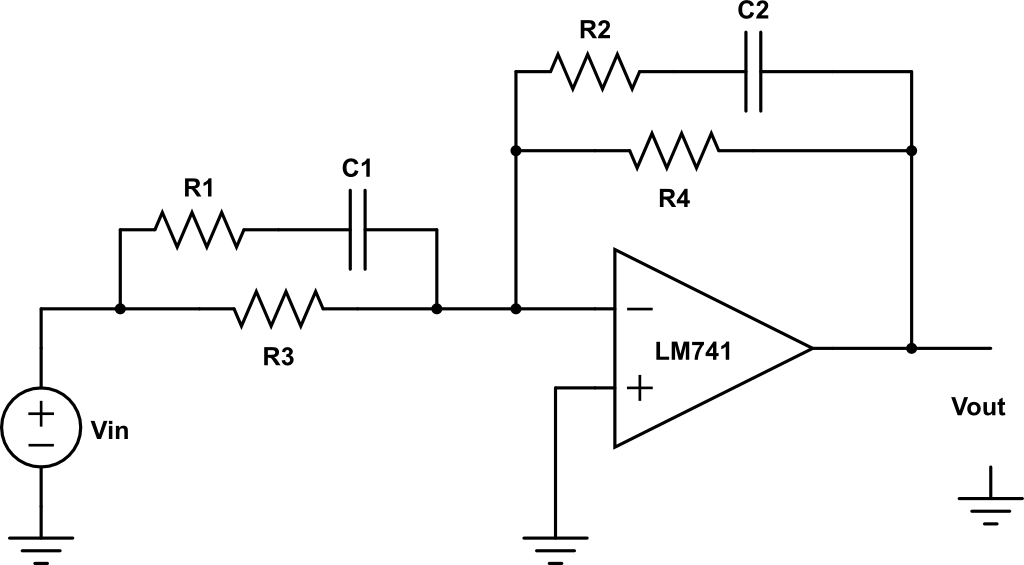
\includegraphics[width=10cm]{q1_circuitDiagram.png}
\end{center}
\caption{A lead-lag compensator circuit diagram for question 1.}
\label{q1_a}
\end{figure}

\subsection*{b}
If we consider the impedance of the group $R_1$, $C_1$ and $R_3$ as $Z_1$ and the impedance of the group  $R_2$, $C_2$ and $R_4$ as $Z_2$, we can get the circuit diagram seen in figure \ref{q1_b}.This circuit essentially operates as an inverting amplifier and hence the relationship between the output and input is given as:
\begin{figure}[h]
\begin{center}
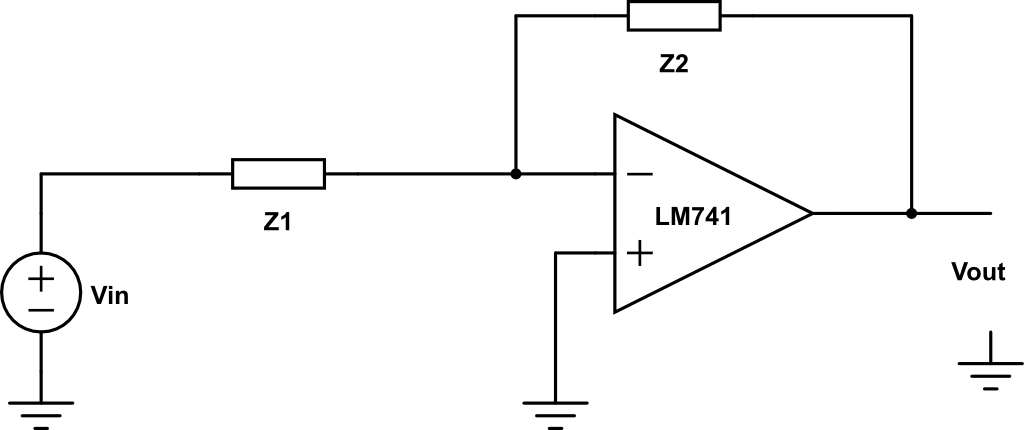
\includegraphics[width=10cm]{revised-lead-lag-simplified.png}
\end{center}
\caption{Simplified lead-lag compensator circuit diagram.}
\label{q1_b}
\end{figure}
 

$$\frac{V_{out}(s)}{V_{in}(s)} = - \frac{Z_2}{Z_1}$$
Where:
$$Z_1 = \frac{R_3 * (R_1 + (1/sC_1))}{R_3 + (R_1 + (1/sC_1))} = \frac{R_3(sR_1C_1 +1)}{s(R_1C_1 + R_3C_1) + 1} \ \text{, and}$$
$$Z_2 = \frac{R_4 * (R_2 + (1/sC_2))}{R_4 + (R_2 + (1/sC_2))} = \frac{R_4(sR_2C_2 +1)}{s(R_2C_2 + R_4C_2) + 1}$$
Thus the gain of the system can now be re-written as:
$$\frac{V_{out}(s)}{V_{in}(s)} = -  \frac{R_4(sR_2C_2 +1)}{(s(R_2C_2 + R_4C_2) + 1)}\frac{(s(R_1C_1 + R_3C_1) + 1)}{R_3(sR_1C_1 +1)} $$
$$=  -  \frac{R_4}{R_3}\frac{(sR_2C_2 +1)}{(s(R_2C_2 + R_4C_2) + 1)}\frac{(s(R_1C_1 + R_3C_1) + 1)}{(sR_1C_1 +1)} $$

We see that the op-amp operates as an inverting amplifier. In order to match the required transfer function, we need to account for the additional $-\frac{R_4}{R_3}$ gain, which we can do by passing the output of the circuit through another inverting amplifier which has a gain of $-\frac{R_3}{R_4}$\footnote{For practical purposes this second op-amp is implemented in LabView as a negative gain.}. Comparing our final transfer function with what is asked in the question, we get:

$$\Big( -  \frac{R_4}{R_3} \times -\frac{R_3}{R_4} \Big)\frac{(sR_2C_2 +1)}{(s(R_2C_2 + R_4C_2) + 1)}\frac{(s(R_1C_1 + R_3C_1) + 1)}{(sR_1C_1 +1)}  = \frac{(1+0.1s)(1 + 5s)}{(1+0.01s)(1 + 10s)}$$

Comparing the LHS and the RHS, we see:
$$R_1C_1 = 0.01$$
$$R_2C_2 = 5$$
$$R_1C_1 + R_3C_1 = 0.01 + R_3C_1 = 0.1$$
$$\implies R_3C_1 = 0.09$$
$$R_2C_2 + R_4C_2 = 5 + R_4C_2 = 10$$
$$\implies R_4C_2 = 5$$
$$\therefore R_4 = R_2$$

\subsection*{c}
While building this circuit, we made the following assumptions:
\begin{itemize}
\item We are using an ideal op-amp, i.e. the input impedance is infinite and the output impedance is negligible. This implies that the op-amp does not load it's input circuit and loading effects are not seen on the op-amps output terminal.

\item The voltage at the non-inverting terminal is equal to the voltage at the non-inverting terminal.

\item The open loop op-amp gain is infinite.

\item The op-amp will operate in an ideal manner when the output is not saturated above or below its supply limits.

\item We used potentiometers to tune the resistors to their required value but none of the components used were ideal components. But for the most part we assumed the values of the resistors were accurate and that capacitors had negligible internal resistance.

\end{itemize}

\subsection*{d}
We can determine the ratings of the components by arbitrarily setting $C_1$ and $C_2$. We set the capacitances because the values available to us is limited whereas we have significantly more flexibility with choosing resistances. By fixing $C_1$ and $C_2$ we find:
$$R_1 = \frac{0.01}{C_1}$$
$$R_2 = \frac{5}{C_2}$$
$$R_3 = \frac{0.09}{C_1} \ \text{,  and}$$
$$R_4 = R_2$$

We additionally see that the gain of the inverting op-amp lead-lag circuit is proportional to $ \frac{R_4}{R_3}$. We  want to limit this so that the output does not get saturated wile trying to amplify the signal by a large amount. As we need to use an input amplitude of up to 2V in part (\emph{i}), for a input supply of +/- 15V, we would like to limit the op-amp output to +/- 10V. Hence we want the gain,$ \frac{R_4}{R_3}, \approx 5$. 

$$\frac{R_4}{R_3} \approx 5 \implies \frac{(5/C_2)}{(0.09/C_1)} \approx 5$$
$$\therefore \frac{C_1}{C_2} = 0.09$$

\xxx{For this circuit we chose $C_1$ = BLALALALAL}, hence ratings of the other components became:
\begin{table}[hbt]
\begin{center}
    \begin{tabular}{|c|c|c|}
        \hline
        \textbf{Component Name} & \textbf{Component Type} & \textbf{Component Specification} \\ \hline
       $ C_1$                     & \text{Electrolytic Capacitor}         & $ \ \mu F     $             \\ 
       $ C_2 $                   & \text{Electrolytic Capacitor}         & $ \ \mu F     $               \\ 
       $ R_1  $                  & \text{Resistor}         & $ \ K\Omega            $        \\ 
       $ R_2 $                    & \text{Resistor}         & $ \ K\Omega        $            \\        
       $ R_3 $                   & \text{Resistor}         & $\ K\Omega   $                 \\ 
       $ R_4$                     & \text{Resistor}         &$ \ K\Omega$                    \\
        \hline
    \end{tabular}
\end{center}
\end{table}

\subsection*{e} Physical implementation.

\subsection*{f}

\subsection*{g}

\subsection*{h}

\subsection*{i}

\subsection*{j}

\section*{Question 2}

\subsection*{a}
The circuit diagram can be seen in figure \ref{q2_a}.
\begin{figure}[h]
\begin{center}
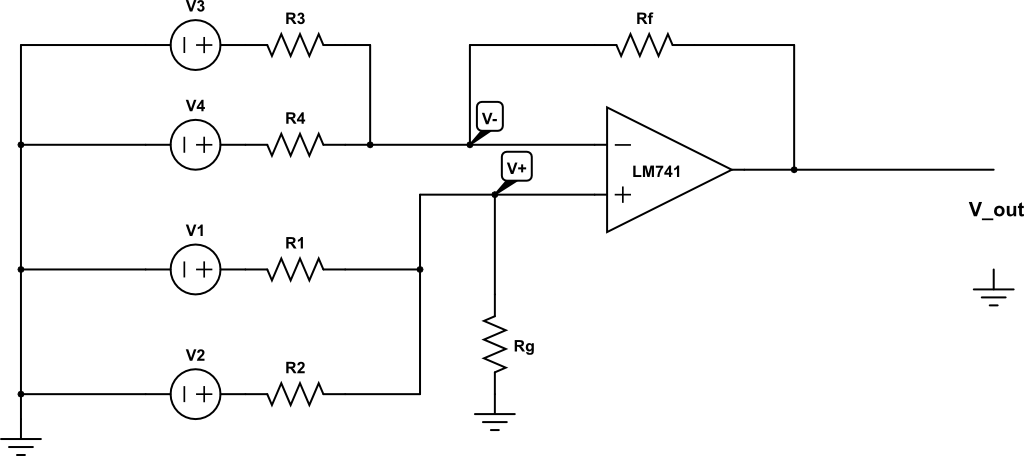
\includegraphics[width=10cm]{q2_circuitDiagram.png}
\end{center}
\caption{The required circuit diagram for question 2.}
\label{q2_a}
\end{figure}


\subsection*{b}
Circuit analysis:\\

At the non-inverting terminal, we effectively have a circuit represented by figure \ref{q2_b1}. We can use Kirchoff's voltage law along with the superposition theorem, we see:
\begin{figure}[h]
\begin{center}
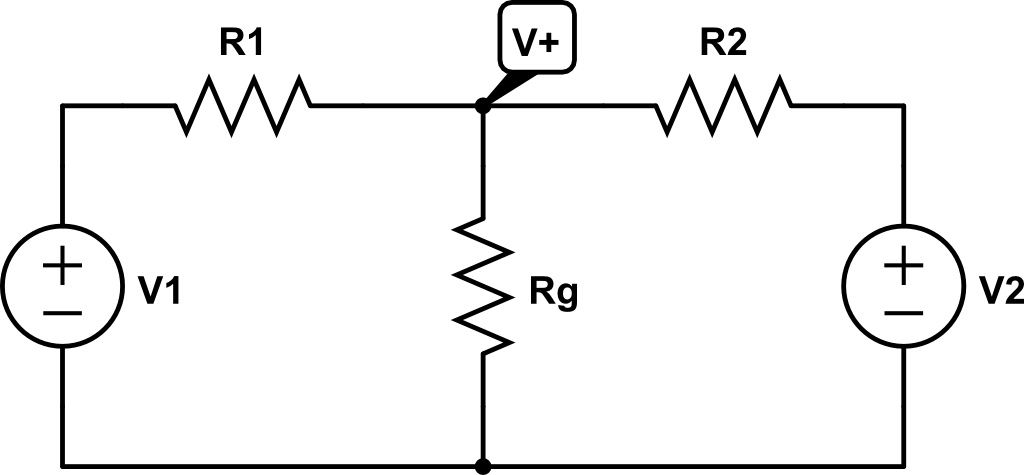
\includegraphics[width=6cm]{lab1_q2_kvl1.png}
\end{center}
\caption{Equivalent circuit at the non-inverting terminal}
\label{q2_b1}
\end{figure}

$$\text{Voltage at $V^+$ due to $V_1$, $V^+_1$, is given by:}$$
$$V^+_1 = \frac{\frac{R_2 R_g}{R_2+R_g}}{R_1 + \frac{R_2 R_g}{R_2+R_g}}\ V_1$$
$$\therefore V^+_1 = \Big(\frac{1}{\frac{R_1}{R_g} + \frac{R_1}{R_2} + 1}\Big) \ V_1$$

$$\text{Similarly, voltage at $V^+$ due to $V_2$, $V^+_2$, is given by:}$$
$$V^+_2 = \frac{\frac{R_1 R_g}{R_1+R_g}}{R_2 + \frac{R_1 R_g}{R_1+R_g}}\ V_2$$
$$\therefore  V^+_2 = \frac{1}{\frac{R_2}{R_g} + \frac{R_2}{R_1} + 1} \ V_2$$

$$\text{Using the superposition theorem to recombine the values, we find that $V+$ is given by:}$$
$$V^+ = V^+_1 + V^+_2 $$
$$V^+ = \frac{1}{\frac{R_1}{R_g} + \frac{R_1}{R_2} + 1} \ V_1 + \frac{1}{\frac{R_2}{R_g} + \frac{R_2}{R_1} + 1} \ V_2 $$

We can now move on to the inverting terminal of the op-amp. The corresponding equivalent circuit is shown in figure \ref{q2_b2}.  Analyzing this circuit, we see that:
\begin{figure}[h]
\begin{center}
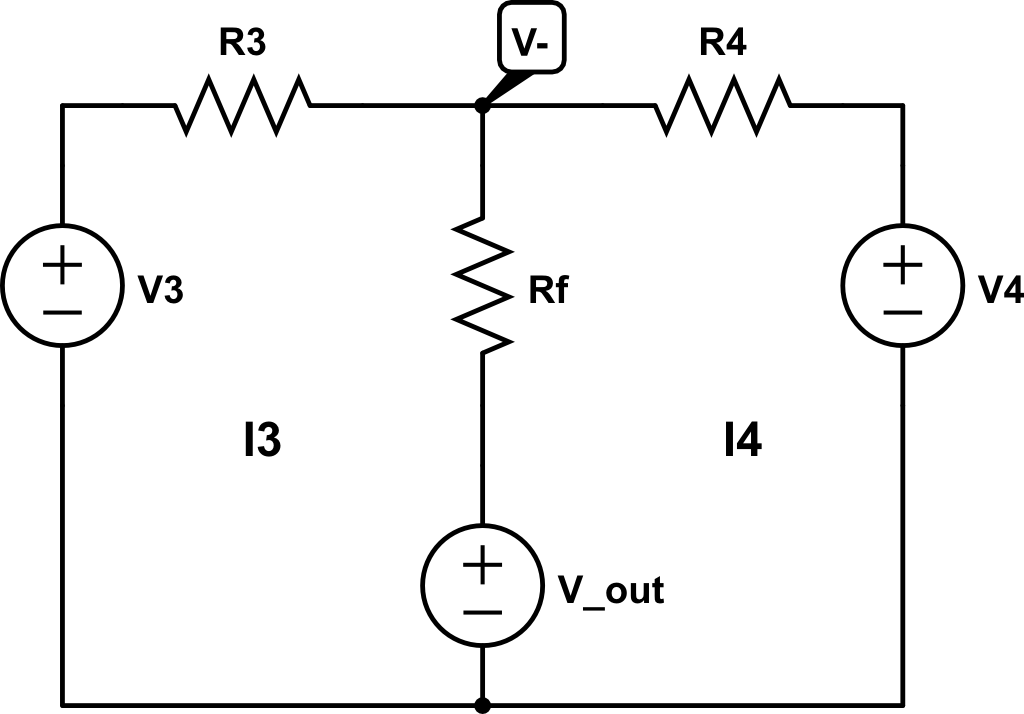
\includegraphics[width=6cm]{lab1_q2_kvl2.png}
\end{center}
\caption{Equivalent circuit at the non-inverting terminal}
\label{q2_b2}
\end{figure}
$$I_3R_3 = V_3 - V^-$$
$$I_4R_4 = V_4 - V^-$$
$$V^- - V_{out} = (I_3 + I_4)R_f $$
$$\text{Substituting from the above equations, we get:}$$
$$ V^- - V_{out} = \Big( \frac{ V_3 - V^-}{R_3} + \frac{ V_4 - V^-}{R_4}\Big) \ R_f$$
$$\text{Reordering the terms, we get:}$$
$$V_{out} =V^- -  \Big( \frac{ V_3 - V^-}{R_3} + \frac{ V_4 - V^-}{R_4}\Big) \ R_f $$
$$\implies V_{out} =V^- \Big( \frac{R_f}{R_3} + \frac{ R_f}{R_4} + 1\Big) - \Big( \frac{R_f}{R_3}\Big)V_3 - \Big( \frac{ R_f}{R_4}\Big)V_4$$

We also know that for an ideal op-amp, $V^+ = V^-$, hence we get:
$$ V_{out} = \Big( \frac{R_f}{R_3} + \frac{ R_f}{R_4} + 1\Big) \Big( \frac{1}{\frac{R_1}{R_g} + \frac{R_1}{R_2} + 1}\Big) V_1 + \Big( \frac{R_f}{R_3} + \frac{ R_f}{R_4} + 1\Big) \Big( \frac{1}{\frac{R_2}{R_g} + \frac{R_2}{R_1} + 1} \Big) V_2 - \Big( \frac{R_f}{R_3}\Big)V_3 - \Big( \frac{ R_f}{R_4}\Big)V_4$$

This is equation is the mathematical representation of the problem statement which which required $V_{out} = a_1V_1 + a_2 V_2 - a_3 V_3 - a_4 V_4$, i.e. :
$$a_1 =  \Big( \frac{R_f}{R_3} + \frac{ R_f}{R_4} + 1\Big) \Big( \frac{1}{\frac{R_1}{R_g} + \frac{R_1}{R_2} + 1}\Big) = 1$$
$$a_2 =  \Big( \frac{R_f}{R_3} + \frac{ R_f}{R_4} + 1\Big) \Big( \frac{1}{\frac{R_2}{R_g} + \frac{R_2}{R_1} + 1} \Big) = 2$$
$$a_3 = \Big( \frac{R_f}{R_3}\Big) = 3$$
$$a_4 = \Big( \frac{ R_f}{R_4}\Big) = 4$$


\subsection*{c}
\xxx{[DO WE HAVE ANY MORE??]}\\
While building this circuit, we made the following assumptions:
\begin{itemize}
\item We are using an ideal op-amp, i.e. the input impedance is infinite and the output impedance is negligible. This implies that the op-amp does not load it's input circuit and loading effects are not seen on the op-amps output terminal.

\item The voltage at the non-inverting terminal is equal to the voltage at the non-inverting terminal.

\item The open loop op-amp gain is infinite.

\item The op-amp will operate in an ideal manner when the output is not saturated above or below its supply limits.

\item We used potentiometers to tune the resistors to their required value but none of the components used were ideal components. But for the most part we assumed the values of the resistors were accurate and that capacitors had negligible internal resistance.

\end{itemize}

\subsection*{d}
We started by choosing $R_f$, $R_g$ and $R_g$ to arbitrary resistances such that they were large enough to make sure that other resistances in the circuit were not small. By this we mean that the values of the other resistances were in the order of Kilo-Ohms. From section \textbf{b}, we can rewrite gains $a_1$ and $a_2$ in terms of $a_3$ and $a_4$ as follows:
$$a_1 =  \Big( a_3 + a_4 + 1\Big) \Big( \frac{1}{\frac{R_1}{R_g} + \frac{R_1}{R_2} + 1}\Big) = 1$$
$$ =  (8) \Big( \frac{1}{\frac{R_1}{R_g} + \frac{R_1}{R_2} + 1}\Big) = 1$$
We can rewrite this  as:
$$8R_2R_g = R_1R_2 + R_1R_g $$
$$\implies R_g = \frac{R_1R_2}{7R_2 - R_1}$$
Similarly for $a_2$, we see:
$$a_2 =  \Big(  a_3 + a_4  + 1\Big) \Big( \frac{1}{\frac{R_2}{R_g} + \frac{R_2}{R_1} + 1} \Big) = 2$$
$$ =  ( 8) \Big( \frac{1}{\frac{R_2}{R_g} + \frac{R_2}{R_1} + 1} \Big) = 2$$
We can re-arrange and re-write the above equations as:
$$R_g = \frac{R_1R_2}{3R_1 - R_2}$$
Equating the two equations which equal $R_g$, we get:
$$ \frac{R_1R_2}{7R_2 - R_1} = \frac{R_1R_2}{3R_1 - R_2}$$
Thus, we get:
$$R_2 = \frac{R_1}{2}$$
Thus we arbitrarily chose $R_f = R_g = 10 \ K\Omega$ and $R_1 = 50 \ K\Omega$
We ended up using the following components in our circuit:
\begin{table}[hbt]
\begin{center}
    \begin{tabular}{|c|c|c|}
        \hline
        \textbf{Component Name} & \textbf{Component Type} & \textbf{Component Specification} \\ \hline
       $ R_f  $                  & \text{Resistor}         & $9.880 \ K\Omega            $        \\ 
       $ R_g $                    & \text{Resistor}         & $9.860 \ K\Omega        $            \\ 
       $ R_1$                     & \text{Resistor}         & $49.3 \ K\Omega        $             \\ 
       $ R_2 $                   & \text{Resistor}         & $24.65 \ K\Omega     $               \\ 
       $ R_3 $                   & \text{Resistor}         & $3.293 \ K\Omega   $                 \\ 
       $ R_4$                     & \text{Resistor}         &$ 2.470 \ K\Omega$                    \\
        \hline
    \end{tabular}
\end{center}
\end{table}

\subsection*{e} Physical implementation.

\subsection*{f} \xxx{John}

\subsection*{g} \xxx{John}

\subsection*{h} 
The beating signal is achieved as a sinusoidal wave which has an amplitude that also varies sinusoidally. In effect, the output is $\sin(\omega_a t)\sin(\omega_b t) $. We can use trigonometric identities to rearrange this sinusoidal product as a sum as follows:
$$\sin(\omega_a t)\sin(\omega_b t) = \frac{\cos(\omega_a t + \omega_b t) - \cos(\omega_a t + \omega_b t)}{2}$$
We use the product-to-sum identity to break up the product of the sines into a sum of cosines. We can again rewrite the cosines in terms of sines by taking into account the phase difference.
$$\frac{\cos(\omega_a t + \omega_b t) - \cos(\omega_a t + \omega_b t)}{2} = \frac{\sin((\omega_a t + \omega_b t) + \pi/2)- \sin((\omega_a t + \omega_b t) + \pi/2)}{2}$$

This way, we can achieve a beating signal as a sum of sinusoids. For the purposes of this question, we chose $\omega_a = 1$ and $\omega_b = 10$ The values for each of the output terminals is as follows:
\begin{table}[h]
\begin{center}
    \begin{tabular}{|c||c|c|c|c|}
        \hline
        ~                 & V1              & V2 & V3              & V4 \\ \hline \hline
        Amplitude (Volts) & 3               & 0  & 1               & 0  \\ \hline
        Frequency (Hz)    & -9              & 0  & 11              & 0  \\ \hline
        Offset (Volts)    & 0               & 0  & 0               & 0  \\ \hline
        Phase (Radians)            & $\frac{\pi}{2}$ & 0  & $\frac{\pi}{2}$ & 0  \\
        \hline
    \end{tabular}
\end{center}
\end{table}

The required LabView screen shot can be seen in figure \ref{q2_h}

\begin{figure}[h]
\begin{center}
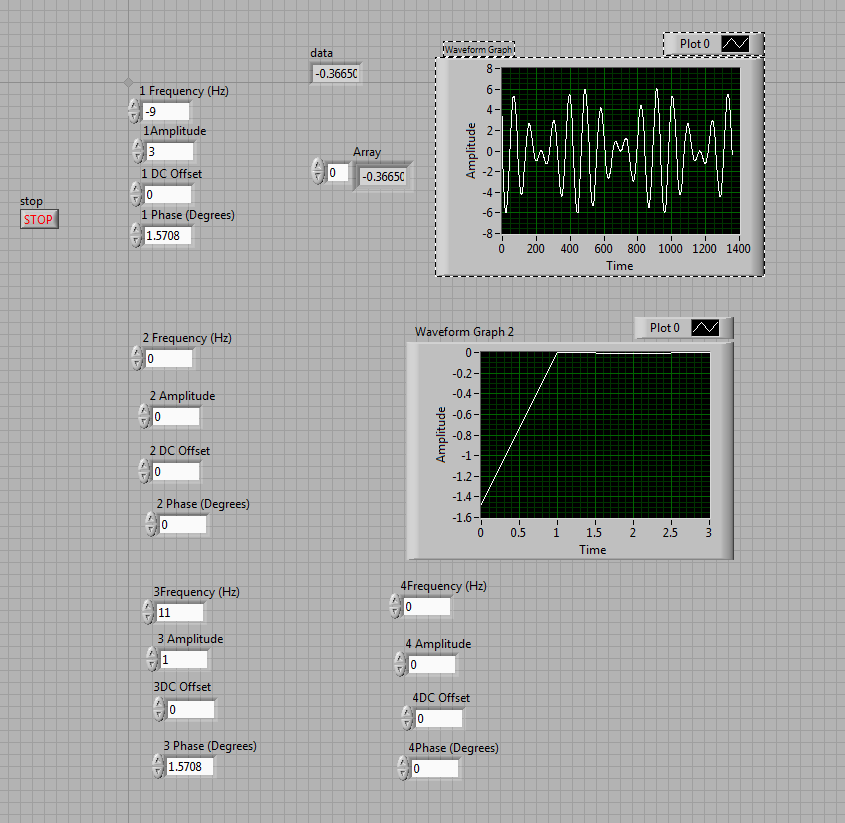
\includegraphics[width=15cm]{problem2_h.png}
\end{center}
\caption{The LabView front-end of a system that produces $\sin(\omega_a t_a)\sin(\omega_b t_b) $.}
\label{q2_h}
\end{figure}
\end{document}


\def\therefore{\boldsymbol{\text{ }
\leavevmode
\lower0.4ex\hbox{$\cdot$}
\kern-.5em\raise0.7ex\hbox{$\cdot$}
\kern-0.55em\lower0.4ex\hbox{$\cdot$}
\thinspace\text{ }}}
